\documentclass{scrartcl}
\usepackage[headsepline]{scrlayer-scrpage}
\pagestyle{scrheadings}
\usepackage[a4paper, left=3cm, right=3cm, top=3cm]{geometry}
\usepackage[english]{babel}
\usepackage{amsmath,amssymb}
\usepackage{graphicx}
\usepackage{float}
\usepackage{hyperref}
\usepackage{url}
\usepackage{csquotes}
\usepackage{caption}
\usepackage{subcaption}
\usepackage{fancyvrb}

\title{Final Exam 1}
\subtitle{Case 1, double real}
\author{Jan Kruska \\ jan.kruska@rwth-aachen.de}
\date{\today}
%\publishers{Platz für Betreuer o.\,ä.}% optional
\ihead{Jan Kruska}
\chead{HPMC - Final Exam 1}
\ohead{\today}

\MakeOuterQuote{"}

\begin{document}
	
	\maketitle
	
	
	\section{Question 1}
	\subsection{Versions}
	\begin{verbatim}
		gcc version 10.1.0 (GCC)
		
		Intel MKL:
		Major version:           2019
		Minor version:           0
		Update version:          1
		Product status:          Product
		Build:                   20180928
		Platform:                Intel(R) 64 architecture
		Processor optimization:  Intel(R) Advanced Vector Extensions 512 (Intel(R) AVX-512) enabled processors
		================================================================
	\end{verbatim}
	
	\subsection{Approach}
	
	First it was observed that the computation of Case 1 could be separated into two parts, the calculation of $Y_i = \frac{1}{2}A_iB_i$ and the calculation of $C_i = B_i^TY_i + Y_i^TB_i$.
	Since the $Y_i$ result is reused it makes sense to calculate it separately to avoid computing it multiple times.
	Since $A_i$ is always symmetric we can use the dsymm BLAS routine to calculate $Y_i$ and save roughly half of the FLOP.
	Furthermore, the second term is very clearly a symmetric rank 2k update, so we can use the dsyr2k BLAS routine to calculate it and accumulate the result in $C$.
	
	The \emph{dcase1} method was implemented in that way, taking the parameter $m$ and calculating the given sum.
	
	Since \emph{dsyr2k} only returns an upper triangular matrix, it is also necessary to re-symmetrize the result again, unless any further procedures can work with symmetric matrices defined only by the upper triangular part.
	
	\section{Question 2}
	See \path{jobs/q2.sh} for script to run experiment and \path{data/q2.txt} for output of this experiment.
	All calculations were performed on one node of the CLAIX-18 cluster.
	To perform accurate timings an entire node was always reserved, even if single-thread performance was to be evaluated (avoid caching inconsistencies etc.)
	
	\subsection{Symmetry}
	Since \emph{dsyr2k} only returns an upper triangular matrix, there is not much point in verifying whether the matrix is actually symmetric as this property was manually enforced.
	
	main.c:
	\begin{verbatim}
		resymmetrize(m, m, C, ldC, 'u');
	\end{verbatim}
	
	utils.c:
	\begin{Verbatim}[tabsize=2]
		void resymmetrize(int m, int n, double *ap, int lda, char uplo)
		{
			int i, j;
			if (uplo == 'u')
			{
				#pragma omp parallel for private(i, j)
				for (j = 0; j < n; j++)
				{
					for (i = j + 1; i < n; i++)
					{
						A(i, j) = A(j, i);
					}
				}
			}
			else if (uplo == 'l')
			{
				#pragma omp parallel for private(i, j)
				for (j = 0; j < n; j++)
				{
					for (i = j + 1; i < n; i++)
					{
						A(j, i) = A(i, j);
					}
				}
			}
		}
	\end{Verbatim} 
	
	\subsection{Time to Solution}
	
	The best time to solution over 10 repetitions for $m=1000$ was $0.056589s$ using a single OpenMP thread.
	
	\subsection{Fraction of Peak Performance}
	The Intel Xeon Platinum 8160, has a clock speed of $2.1$GHz and two AVX512 FMA units.
	As such the peak performance for one core defined as 
	\begin{equation}
		R_{peak} = clock speed \cdot \frac{unit width}{word width} \cdot \#fpunits \cdot \#flop/instruction
	\end{equation}
	results is $2.1e9 \cdot \frac{512}{64} \cdot 2 \cdot 2 = 67.2e9$ FLOPS, or $67.2$ GFLOPS.
	This is seemingly backed up by other benchmarks, e.g. the \href{https://www.top500.org/system/179574/}{CRESC06} supercomputer equipped with the same processor that reaches the same per-core peak performance.
	Surprisingly both my program (main.c) and a simple dgemm (dgemm.c) both seem to beat that benchmark, which should be physically impossible.
	
	The reason for that could be that I missed some components in the specification, which seems unlikely since there are other benchmarks that back up our calculations.
	It may be possible that the so-called "Intel® Turbo Boost Technology" is responsible for this discrepancy and the actual single-core frequency that should be used is $3.7$GHz, which would result in $2.1e9 \cdot \frac{512}{64} \cdot 2 \cdot 2 = 118.4e9$ FLOPS.
	This would be more realistic given the results presented below, however, I am unsure when and how a core reaches the so-called "Turbo Frequency".
	Since this is the only explanation I was able to come up with, and the only number for which the results below make sense I will proceed using it as peak performance for any future comparisons.
	
	Taking this number as peak performance the mean fraction of peak performance was $\frac{83.6210}{118.4}=0.71$.
	
	\section{Question 3}
	\subsection{Preliminaries}
	See \path{jobs/q3.sh} for script to run experiment and \path{data/q3.csv} for output of this experiment.
	See \path{dgemm.c}, \path{jobs/dgemm.sh} and \path{data/dgemm.txt} for the dgemm reference measurement.
	All calculations were performed on one node of the CLAIX-18 cluster.
	To perform accurate timings an entire node was always reserved, even if single-thread performance was to be evaluated (avoid caching inconsistencies etc.)
	
	Note that the results for 5 repetitions varied strongly, and no clear patterns were discernible, so the simulation was also run for 50 iterations, which seemed to produce much more stable values.
	These results can be found in \path{data/q3-50.csv}.
	
	\subsection{Results 5 repetitions}
	\begin{figure}[h]
		\centering
		\begin{subfigure}[b]{0.49\textwidth}
			\centering
			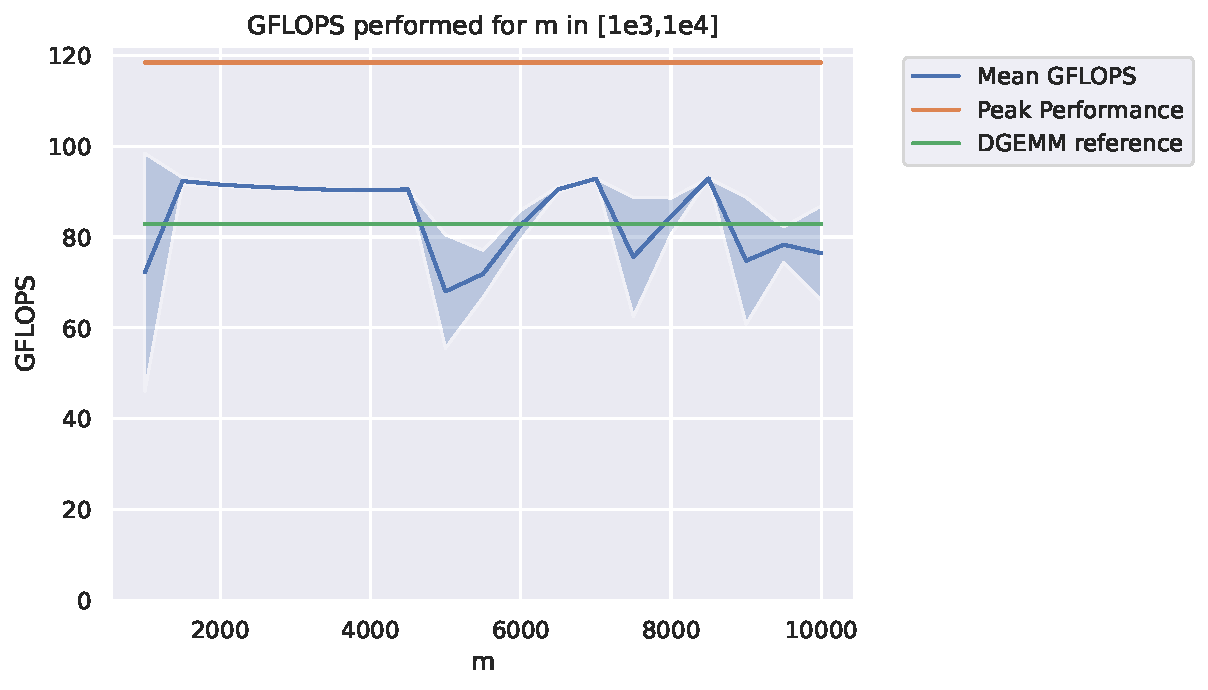
\includegraphics[width=\textwidth]{../plots/q3}
			\caption{5 repetitions}
			\label{fig:q3-5}
		\end{subfigure}
		\hfill
		\begin{subfigure}[b]{0.49\textwidth}
			\centering
			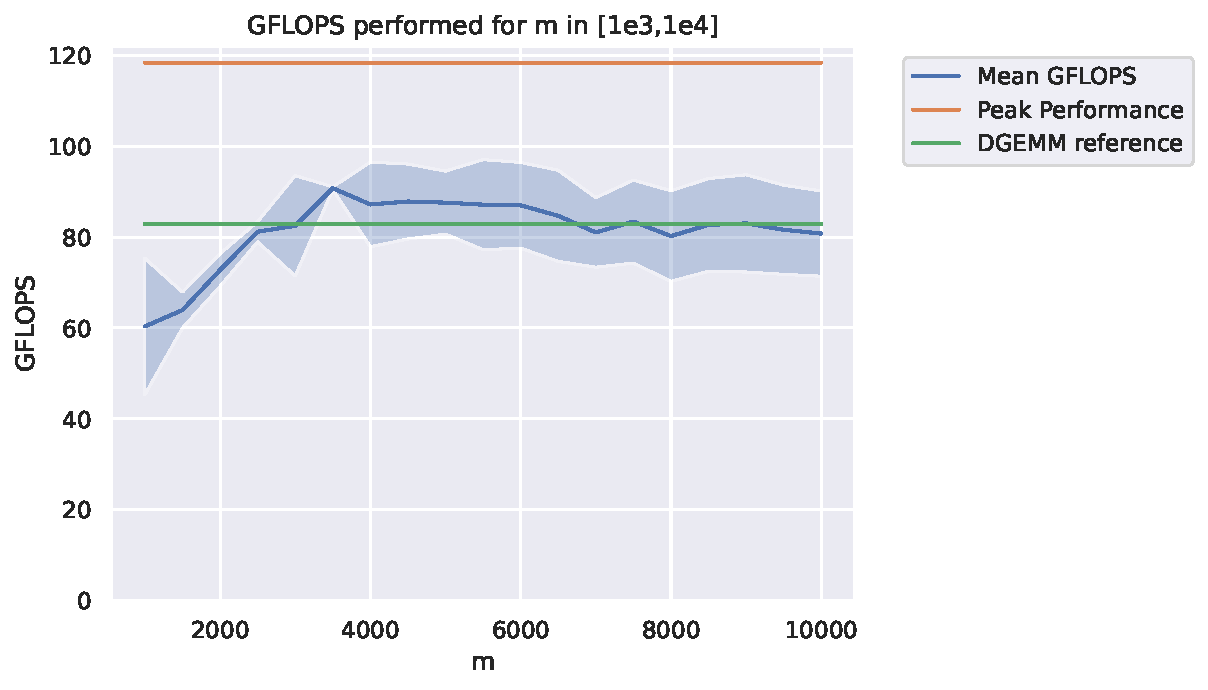
\includegraphics[width=\textwidth]{../plots/q3-50}
			\caption{50 repetitions}
			\label{fig:q3-50}
		\end{subfigure}
		\caption{GFLOPS performed for different $m$}
		\label{fig:q3}
	\end{figure}
	Mean GFLOPS performed as well as standard deviation bands are displayed. 
	For reference, the theoretical peak performance of the systems given a clock speed of $3.7$GHz and the GFLOPS performed by the dgemm routine for the multiplication of two square $1000 \times 1000$ matrices is shown.
	
	In terms of actual trends, the results are surprisingly inexpressive, no consistent trend w.r.t. the parameter $m$ can be seen.
	Mostly the performance seems to hover around the performance of DGEMM at around 80 GFLOPS, sometimes above it at around 90 GFLOPS, sometimes a bit below it at around 70 GFLOPS.
	The largest matrix we encounter in the routine is the matrix $C$, which is $m \times m$.
	Since $n \ll m$ the size of matrices $A, B, Y$ can be neglected for this analysis.
	For the smallest $m$ the matrix $C$ has a million entries, however since we use a symmetric rank 2k update only half of these are ever read and written.
	This means for the smallest $m$ the effectively used portions of $C$ take up 4MB, exceeding both the L1 and L2 caches of the given CPU.
	Up until $m=3000$ the used entries of matrix $C$ still fit into the L3 cache, yet there is no marked drop in performance.
	All of this suggests that the size of the matrix $C$ has little influence on the performance of the algorithm for $m \in [1000;10000]$.
	
	The next smaller class of matrices are the $n \times m$ matrices $B$ and $Y$.
	These range between 1e5 and 3e6 elements, leading to memory needs between 800KB and 24MB, so even in the smallest case, both will not fit into the L1 or L2 cache together.
	The size of the matrices $B$ and $Y$ could be the reason for the drop in performance on the high end of the spectrum since the matrices start to not fit into the L3 cache anymore, however, this is already the case for $m=8000$, after which another peak occurs.
	
	The smallest matrices occurring in this calculation are the matrices $A_i$ ranging from 1e4 to 9e4 elements, resulting in memory need between 40KB and 350KB.
	However, since these remain the same independent of $m$ and their sizes are negligible it seems unlikely that they would have a significant impact on the observed behavior in the figure.
	
	\subsection{Results 50 repetitions}
	As already stated the results obtained from just 5 repetitions varied strongly between experiments.
	As such one with 50 repetitions was performed, which seems much more stable.
	Most of the analyses of the previous part regarding matrix sizes still hold, notably that most of the matrices are both too large for the lower caches, but not sufficiently large to cause significant cache misses in the L3 cache.
	Interestingly the performance seems worse for lower values of $m$. 
	I would attribute that to the fact that the actual runtime for the procedure is in the tenths of seconds, which means overhead from constant factors, like sanity checks and method calls can easily form a significant portion of the work.
	As $m$ rises more and more of the work performed are actually matrix computations, and thus the performance rises to roughly match that of \emph{dgemm}.
	As opposed to the five repetition example, mean and standard deviation seem to behave much better here, though the mean slowly declines with larger $m$.
	As noted previously from $m=3000$ onwards the $m\times m$ triangle matrices do not fit into the L3 cache anymore, which leads to more and more cache misses.
	
	\section{Question 4}
	See \path{jobs/q4.sh} for script to run experiment and \path{data/q4.csv} for output of this experiment.
	All calculations were performed on one node of the CLAIX-18 cluster.
	To perform accurate timings an entire node was always reserved, even if single-thread performance was to be evaluated (avoid caching inconsistencies etc.)
	
	\begin{figure}[h]
		\centering
		\begin{subfigure}[b]{0.49\textwidth}
			\centering
			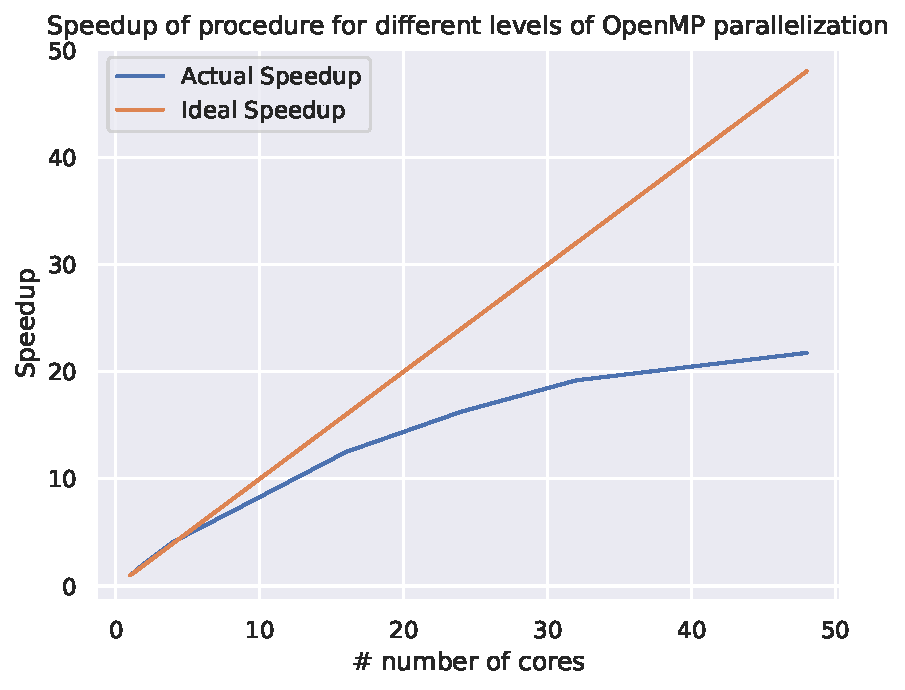
\includegraphics[width=\textwidth]{../plots/q4-speedup}
			\caption{Speedup}
			\label{fig:q4-speedup}
		\end{subfigure}
		\hfill
		\begin{subfigure}[b]{0.49\textwidth}
			\centering
			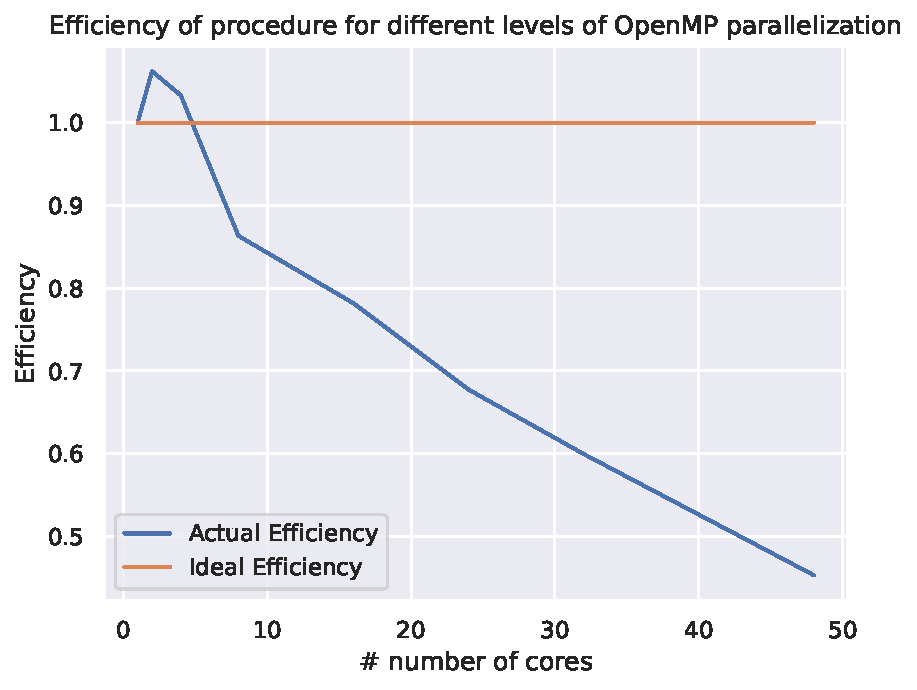
\includegraphics[width=\textwidth]{../plots/q4-efficiency}
			\caption{Efficiency}
			\label{fig:q4-efficiency}
		\end{subfigure}
		\caption{Speedup \& Efficiency for different numbers of cores}
		\label{fig:q4}
	\end{figure}
	
	Overall there is not much interesting to say about the speed-up. 
	It is a very typical graph of sub-linear speed-up, which is to be expected.
	It should be noted that especially for lower numbers of cores ($<16$) the speed-up is still keeping par with the ideal speed-up quite well and for very low numbers of cores it is even super-linear (more clearly visible in the efficiency plot).
	An efficiency of roughly $0.5$ at 48 threads, is however still very good and suggests a highly parallelized application.
	Referencing Amdahl's law, such speed-up would suggest a parallelization proportion above $95\%$, though most of the slow down here is to be due to communication overheads, which need not be entirely sequential.
	
	This test was done with $m=10000$, though the assumption would be that higher values of $m$ would result in higher efficiencies and speedups since we are working with level 3 BLAS routines, i.e. we have a quadratic amount of data with a cubic amount of floating-point operations, which means the proportion of communications to calculation would shrink with larger problem sizes.
	
	It should also be noted, that the drop in efficiency could be due to the processor decreasing its clock speed (or no longer increasing it above the base speed), as more and more cores are used and the power draw increases.
	Again this is somewhat dependent on how the so-called "Intel® Turbo Boost Technology" works specifically, but the latter values seem much more in line with what we would expect, if we take the peak performance using the base clock speed.
	
\end{document}

